%--LECTURE PAGE 41--%
\section{Cryptography}
    \subsection{Introduction to Cryptography}
    \textbf{Cryptography} is the science and study of secret writing, \textbf{cryptoanalysis} is the science and the study of methods of breaking ciphers, \textbf{Cryptology} is cryptography and cryptoanalysis. Today cryptography is the study of mathematical techniques related to aspects of information security such as:
    \begin{itemize}
        \item \textbf{Confidentiality}: encryption algorithms hide the content of messages
        \item data \textbf{Integrity}: integrity check functions provide the means to detect whether a document has been changed
        \item entity authentication 
        \item data origin authentication: message authentication codes or digital signature algorithms provide the means to verify the source and integrity of a message
    \end{itemize}
    Cryptography is a security mechanism that includes a set of techniques for scrambling or disguising data so that is available only to someone who can restore the data to its original form. It provides a string economical basis for offering data security as a security service.
    
    \myparagraph{Cryptosystem}
    A cryptosystem is a 5-tuple (E,D,M,K,C) where
    \begin{itemize}
        \item \textbf{E} is an \textit{encryption} algorithm
        \item \textbf{D} is a \textit{decryption} algorithm
        \item \textbf{M} is the set of \textit{plaintexts}
        \item \textbf{K} is the set of \textit{keys} 
        \item \textbf{C} is the set of \textit{ciphertexts}
    \end{itemize}
    
    So $D(E(m,k),k)=m$, encryption and decryption keys are not necessarily the same (simmetric or asimmetric cryptography).
    
    \textbf{Kerckhoffs principle}: do not rely on the secrecy of algorithms, the key should be the only secret that needs protection
    
    \myparagraph{About Keys}
    A key is an input to a cryptographic algorithm used to obtain confidentiality, integrity and authenticity or other property over some data, security depends on keeping the key secret. Frequent key changes are usually desirable to limit the ammount of data compromised. The stranght of any cryptographic system rests with the \textbf{key distribution technique}.
    
    We say that an encryption scheme is \textbf{computationally secure} if the ciphertext generated by the scheme meets one or booth of the following criteria: the cost of breaking the cipher exceeds the value of the information and the time required to break the cipher exceeds the useful lifetime of the information. We use a \textbf{trapdoor one-way functions}, is a one way function with an additional requirement: the computation in the reverse direction becomes straightforward whene some additional information is revealed.
    
    \subsection{Different type of ciphers}
    \myparagraph{Closer look}
    We have two types of transformations:
    \begin{itemize}
        \item \textbf{Substitution:} each element in the plaintext is mapped into another element.
        \item \textbf{Transportation:} elements in the plaintext are rearranged so there are same letters but arranged in a different order.
    \end{itemize}
    
    \subsubsection{Substitution ciphers}
    In brief substitute one symbol for another, the key is the substitution. A simply substitution cipher is \textbf{Caesar cipher}: every character is replaced with the character e.g. three slots to the right. The key is the number of characters to shift the cipher alphabet. Mathematically speaking: every character is a number $'a' - 0$ and  $ 'b' - 1$ ecc, $e(x) =(x+k) mod 26$ where k is the shift applied. $d(x)=(x-k) mod 26$. This cipher is very easy to attak with a bruteforce (shift has to be between 1 and 25), another approach is to study the letters frequency of each language and then use it to crack the code.
    
    \myparagraph{Vigenere cipher}
    It's a generalization of the Caesar cipher, as it we map letters with numbers. First select a keyword, then write out the keyword repeatedly underneath the plaintext untily every plaintext letter has a keyword letter beneath it. Finally, encrypt each plaintext letter using Caesar cipher, whose key is the number associated with the keyword letter written beneath it. 
    If the length of the keyword is the same as the length of the plaintext, a separate Caesar cipher is used to encrypt each plaintext letter, which makes it impossible to determine the correct plaintext without the key.
    
    \subsubsection{Transposition ciphers}
    In brief is the scramble of symbols to produce output, the key is the permutation of symbols. So the unit in the plaintext are rearranged in a different and usually quite complex order (the units themselves are left unchanged).
    \myparagraph{Columnar cipher}
    In this transportation the message is written out in row of a fixed length, and then read out again column by column. Both the width of the rows and the permutation of the columns are usually defined by a keyword.
    \\Example:      
    \begin{itemize}
        \item Plaintext: We are discovered. Flee at once
        \item Keyword: ZEBRA
    \end{itemize}
    \begin{table}[h!]
        \centering
        \begin{tabular}{c c c c c c}
            Z & E & B & R & A & S\\
            6 & 3 & 2 & 4 & 1 & 5\\
            W & E & A & R & E & D\\
            I & S & C & O & V & E\\
            R & E & D & F & L & E\\
            E & A & T & O & N & C\\
            E & Q & K & J & E & U\\
        \end{tabular}
    \end{table}
   
    So the \textbf{ciphertext} is: EVLNE ACDTK ESEAQ ROFOJ DEECU WIREE
    \\(the last 5 letters are random, not part of the message).
    
    \subsection{Modern cryptography}
    \subsubsection{Simmetric Key Cryptography}
    Symmetric keys is where a single key (k) is used for \textbf{E} and \textbf{D}, all receivers have access to key. This guarantee only confidentiality. There are 2 types of symmetric key crypto
    \myparagraph{Stream ciphers}
    Encrypt a sequence of short data blocks under a changing key stream, the security relies on design of key stream generator (encryption usually simple, performed with a XOR). The main idea is use Vigenere cipher adapted to stream of bits rather than text or letters. Same plaintext bit will encrypt to a different bit every time it is encrypted. This technique is no more used, is very week, was used in real time application like mobile communication (BT) and video streaming.
    \myparagraph{Block ciphers}
    Encrypt sequences of long data blocks without changing the key, the security relies on design of encryption function. They use substitution and transposition adapted to manipulate blocks of bits, a block cipher breaks the message M into successive blocks (M1, M2, ..) and encrypt each block with the same key k. Data Encryption Standard \textbf{(DES} and Advanced Encryption Standard \textbf{(AED)} are well known examples of block cipher systems.
    
    \textbf{Feistel} is a block cipher, it splits the plaintext into two equal-size halves, the round funtion F \textbf{(Substitution)} is applied to one half, using a subkey K. Then the output is XORed with the other half. Then the two halves are then swapped. \textbf{DES} use this technique and has 16 rounds, instead of using the same key in each round, a different subkey is derived from the main key. When decrypting, inverse process. DES was craked by a sort of brute force attack so after this and after almost 5 years \textbf{AES} was created and become the official successor to DES in 2001.
    
    \myparagraph{AES}
    The encryption process is based on a series of table lookups and XOR operations (which are very fast operation to perform on a computer. Decryption process consist of doing the ecryption in reverse order. Nowadays AES is unbreakable but we don't know for how much time it remains safe.
    
    \subsubsection{Asymmetric Key Cryptography}
    It's also called Public Key Cryptography \textbf{(PKC)}, it's a two key crypto system in which two parties could engage in a secure communication over a non-secure communications channel without sharing a secret key. PKC guarantee integrity but not confidentiality and authentication. PKC use one way functions, if we want to be more precise they are trapdoor one way functions because if we know the key (trapdoor) we can easily invert the function.
    \myparagraph{Basic idea}
    Use two key, one to encode and one to decode, they have to be mathematically related although knowledge of one key does not allow someone to easily determine the other key. It does not matter which key is applied first, both keys are required for the process to work.
    
    One of the keys is designated the public keyand may be advertised as widely as the owner wants, the other key is designated the private key and is never revealed to another party. So how to send a message: Alice wants to send Bob a message
    \begin{itemize}
        \item Alice encrypts some indormation using Bobs public key
        \item Bob decrypts the ciphertext using his private key
    \end{itemize}
    Method could be also used to prove who sent a message
    \begin{itemize}
        \item Alice could encrypt some plaintext with her private key
        \item When Bob decrypts using Alice's public key he knows that Alice sent the message and Alice cannot deny having sent the message.
    \end{itemize}
    This last thing create a sort of digital signature that certifies (not totally) who sent the message.
    
    \myparagraph{RSA}
    A famous PKA algorithm used today is \textbf{RSA} (Rivest, Shamir, Adleman) it's used in hundreds of software products for \textbf{key exchange, digital signatures and encryption}. The mathematical trick of RSA is that is relatively easy to compute products compared to computing factorizations. Key-pair is derived from a very large number n that is the product of two prime numbers chosen according to special rules:
    \begin{itemize}
        \item prime may be 100 or more digits in length each
        \item an attacker cannot determine the prime factor of n from this information alone
    \end{itemize}
    Let's explain the algorithm:
    \begin{enumerate}
        \item Let \textit{p} and \textit{q} two large prime numbers
        \item Let \textit{N=p*q} be the \textbf{modulus}
        \item Choose \textit{e} relatively prime to \textit{(p-1)*(q-1)}
        \item Find \textit{d} s.t. \textit{e*d=1mod(p-1)(q-1)}
        \item Set the \textbf{public key} to \textit{(N,e)}
        \item Set the \textbf{private key} to \textit{d}
    \end{enumerate}
    To \textbf{encrypt} plaintext compute $C=M^emodN$, for \textbf{decrypt} compute $M=C^dmodN$.
    
    We can easily check \textbf{integrity} with RSA hashing at first the message and then signing the digest, we send all the signed digest and the message, then when reciving we hash the message recived and verify the signature. With this we can decide if the Integrity is preserved or not.
    
    \begin{figure}[h!]
        \centering
        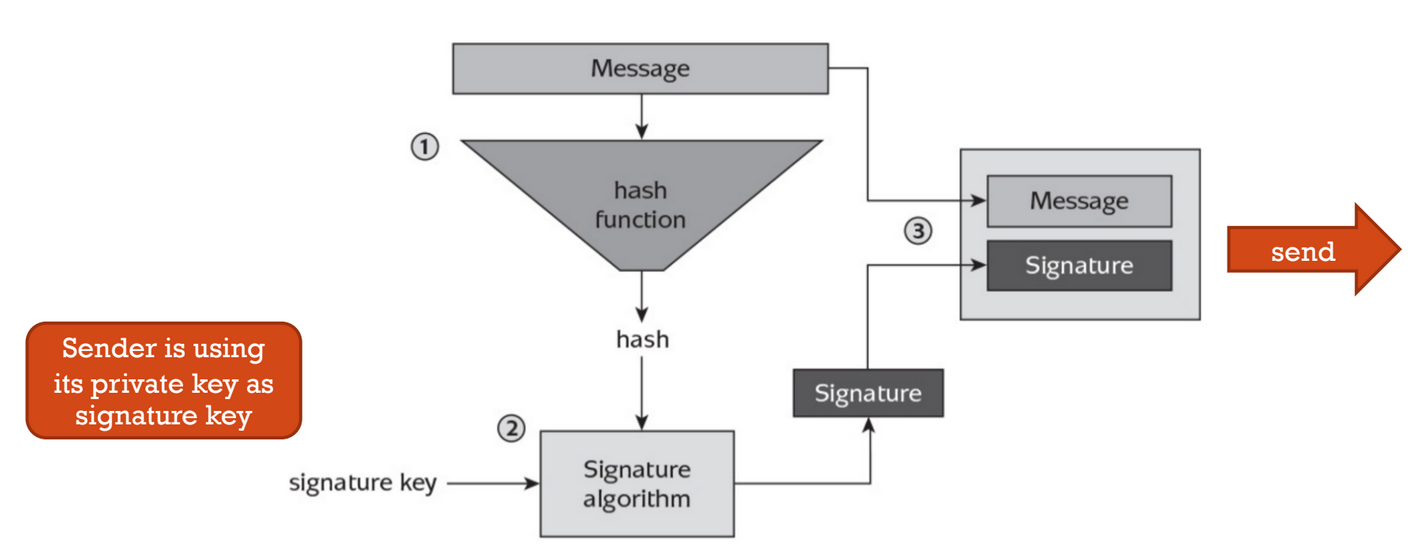
\includegraphics[scale=0.3]{images/intrsa1.png}
    \end{figure}
    
    \FloatBarrier
    
    \begin{figure}[h!]
        \centering
        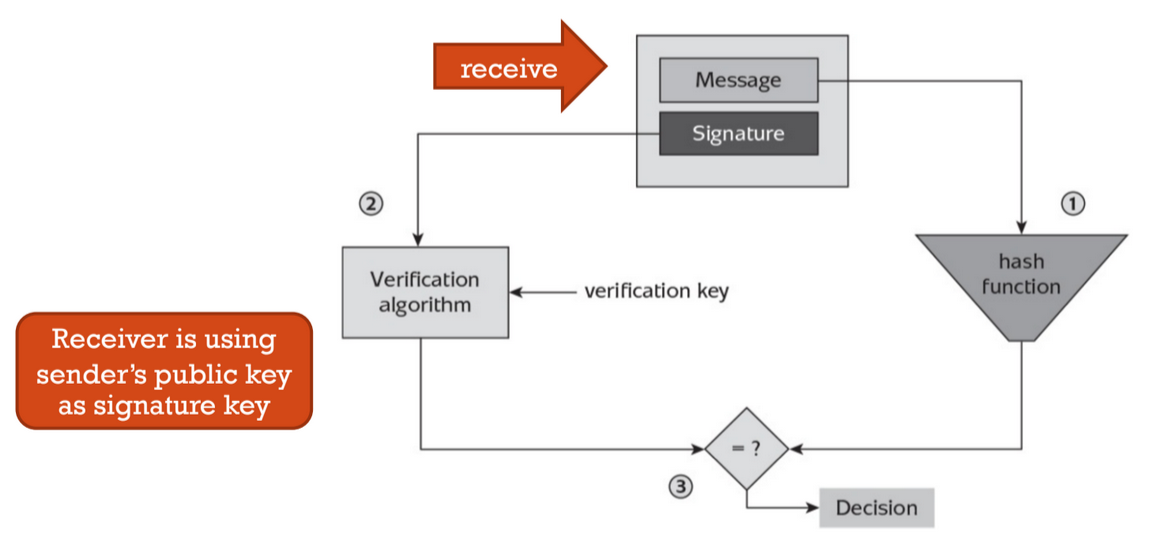
\includegraphics[scale=0.3]{images/intrsa2.png}
    \end{figure}
    
    \FloatBarrier
    
    \myparagraph{DH}
    After the RSA algorithm Diffie and Hellman came up with their own algorithm, \textbf{DH} is used for secret key exchange only, not for authentication or digital signatures. The mathematical trick of DH is that is relatively easy to compute exponents compared to computing discrete logarithms. It allows two parties (e.g. Alice and Bob) to generate a secret key. Mathematical steps:
    \begin{enumerate}
        \item Alice and Bob publicy agree to use a modulus \textit{p}=23 and a base \textit{g}=5 (which is a primitive root modulo 23)
        \item Alice chooses a secret integer \textit{a}=4 then sends Bob $A=g^a mod p$
        \item Bob chooses a secret integer \textit{b}=3 then sends Alice $B=g^b mod p$
        \item Alice computes $s=B^a mod p$
        \item Bob computes $s=A^b mod p$
        \item Alice and Bob now share a secret
    \end{enumerate}
    Where \textbf{A} is the public key of Alice and \textbf{a} is the private key od Alice, \textbf{B} is the public key of Bob and \textbf{b} is the private key of Bob. The security of DH depends on the difficulty of the Discrete Logarithm Problem.
    
    DH does not provide authentication, an attacker C sitting between A and B can mount a Man-In-The-Middle (MITM) attack. The problem now is to establish the entities involved in the communication